%%%%%%%%%%%%%%%%%%%%%%%%%%%%%%%%%%%%%%%%%
% Beamer Presentation
% LaTeX Template
% Version 1.0 (10/11/12)
%
% This template has been downloaded from:
% http://www.LaTeXTemplates.com
%
% License:
% CC BY-NC-SA 3.0 (http://creativecommons.org/licenses/by-nc-sa/3.0/)
%
%%%%%%%%%%%%%%%%%%%%%%%%%%%%%%%%%%%%%%%%%

%----------------------------------------------------------------------------------------
%	PACKAGES AND THEMES
%----------------------------------------------------------------------------------------

\documentclass{beamer}

\mode<presentation> {

% The Beamer class comes with a number of default slide themes
% which change the colors and layouts of slides. Below this is a list
% of all the themes, uncomment each in turn to see what they look like.

%\usetheme{default}
%\usetheme{AnnArbor}
%\usetheme{Antibes}
%\usetheme{Bergen}
%\usetheme{Berkeley}
%\usetheme{Berlin}
%\usetheme{Boadilla}
%\usetheme{CambridgeUS}
%\usetheme{Copenhagen}
%\usetheme{Darmstadt}
%\usetheme{Dresden}
%\usetheme{Frankfurt}
%\usetheme{Goettingen}
%\usetheme{Hannover}
%\usetheme{Ilmenau}
%\usetheme{JuanLesPins}
%\usetheme{Luebeck}
\usetheme{Madrid}
%\usetheme{Malmoe}
%\usetheme{Marburg}
%\usetheme{Montpellier}
%\usetheme{PaloAlto}
%\usetheme{Pittsburgh}
%\usetheme{Rochester}
%\usetheme{Singapore}
% \usetheme{Szeged}
%\usetheme{Warsaw}

% As well as themes, the Beamer class has a number of color themes
% for any slide theme. Uncomment each of these in turn to see how it
% changes the colors of your current slide theme.

% \usecolortheme{albatross}
% \usecolortheme{beaver}
% \usecolortheme{beetle}
% \usecolortheme{crane}
% \usecolortheme{dolphin}
% \usecolortheme{dove}
% \usecolortheme{fly}
% \usecolortheme{lily}
% \usecolortheme{orchid}
% \usecolortheme{rose}
% \usecolortheme{seagull}
% \usecolortheme{seahorse}
\usecolortheme{whale}
% \usecolortheme{wolverine}

%\setbeamertemplate{footline} % To remove the footer line in all slides uncomment this line
%\setbeamertemplate{footline}[page number] % To replace the footer line in all slides with a simple slide count uncomment this line

%\setbeamertemplate{navigation symbols}{} % To remove the navigation symbols from the bottom of all slides uncomment this line
}

\usepackage{graphicx} % Allows including images
\usepackage{booktabs} % Allows the use of \toprule, \midrule and \bottomrule in tables
\usepackage[brazil]{babel}
\selectlanguage{brazil}
\languagepath{brazil}
\deftranslation[to=brazil]{Example}{Exemplo}
\deftranslation[to=brazil]{Theorem}{Teorema}
\usepackage[utf8]{inputenc}
\usepackage{amssymb}
\usepackage{mathtools}

%----------------------------------------------------------------------------------------
%	TITLE PAGE
%----------------------------------------------------------------------------------------

\title[Transações]{Transações de SGBDs} % The short title appears at the bottom of every slide, the full title is only on the title page

\author{Ramon Duarte de Melo} % Your name
\institute[UFRJ] % Your institution as it will appear on the bottom of every slide, may be shorthand to save space
{
    Universidade Federal do Rio de Janeiro \\ % Your institution for the title page
    \medskip
    \textit{ramonduarte@poli.ufrj.br} % Your email address
}
\date{\today} % Date, can be changed to a custom date

\begin{document}

\begin{frame} % SLIDE 1
    \titlepage % Print the title page as the first slide
\end{frame}

\begin{frame} % SLIDE 2
    \frametitle{Sumário} % Table of contents slide, comment this block out to remove it
    \tableofcontents % Throughout your presentation, if you choose to use \section{} and \subsection{} commands, these will automatically be printed on this slide as an overview of your presentation
\end{frame}

%----------------------------------------------------------------------------------------
%	PRESENTATION SLIDES
%----------------------------------------------------------------------------------------

%------------------------------------------------
\section{Introdução} % Sections can be created in order to organize your presentation into discrete blocks, all sections and subsections are automatically printed in the table of contents as an overview of the talk
%------------------------------------------------

\subsection{Definições} % A subsection can be created just before a set of slides with a common theme to further break down your presentation into chunks

\begin{frame} % SLIDE 3
    \frametitle{Glossário}
    
    \begin{block}{Recurso}
        Abstração-chave de um pedaço coeso de informação. Dentro do contexto da disciplina de \emph{Bancos de Dados}, consideraremos como um subconjunto qualquer de dados que possa ser nomeado, agrupado, processado ou referenciado: um registro, ou uma coluna, ou mesmo toda a base de dados. 
    \end{block}
    \begin{block}{Cadeado (ou \emph{lock})}
        Estrutura de dados implementada atomicamente pelo sistema operacional que oferece controle de acesso concorrente a um determinado recurso através da exclusão mútua.
    \end{block}
\end{frame}

%------------------------------------------------

\begin{frame} % SLIDE 4
    \frametitle{Glossário}

    \begin{block}{Requisição de cadeado}
        Feitas pela aplicação ao gerenciador de concorrência (\emph{lock manager}). A transação fica bloqueada até que receba o sinal de cadeado concedido.
    \end{block}
    \begin{block}{Cadeado binário}
        Estrutura de dados usada para impedir que qualquer outra aplicação tenha acesso concorrente ao recurso. Não são efetivamente utilizados em sistemas onde múltiplas aplicações executem simultaneamente.
    \end{block}
\end{frame}


\begin{frame} % SLIDE 5
    \frametitle{Glossário}

    \begin{block}{Cadeado exclusivo (\emph{lock X})}
        Similar ao cadeado binário, permite a livre leitura e/ou escrita aplicando exclusão mútua nos sistemas onde acesso compartilhado está disponível.
    \end{block}
    \begin{block}{Cadeado compartilhado (\emph{lock S})}
        Permite somente a leitura, em modo concorrente a outras transações de leitura.
    \end{block}
\end{frame}

%------------------------------------------------

\begin{frame} % SLIDE 6
    \frametitle{Glossário}

    \begin{block}{\emph{Deadlock}}
        Situação em que conflitos de acesso previnem as transações envolvidas de chegarem a um acordo em que ambas possam obter os recursos necessários para prosseguirem.
    \end{block}
    \begin{block}{Granularidade}
        Porção da base de dados que um único recurso pode representar. Uma menor granularidade representa a capacidade do recurso de representar dados de menor extensão.
    \end{block}
\end{frame}

\begin{frame} % SLIDE 7
    \frametitle{Glossário}

    \begin{block}{Serialização}
        Característica de um escalonamento reprodutível num cenário hipotético em que cada transação é mutuamente exclusiva e executada uma após a outra.
    \end{block}
    \begin{block}{Recuperação}
        Característica de um escalonamento que garante que nenhuma de suas transações exija um \emph{rollback} uma vez que concluam com sucesso.
       \end{block}
    \begin{block}{Recuperação estrita}
        Característica de um escalonamento recuperável que prevê uma ordem estrita de \emph{rollbacks} para transações abortadas.
    \end{block}
\end{frame}

%------------------------------------------------
\section{Q9: Protocolos \emph{lock-based}}
% Discuta os protocolos de controle de concorrência baseados em “Locks”,
% mencionando em detalhes o protocolo “\emph{Two-Phase Locking) (2PL)”,
% mencionando Shared/Exclusive (or Read/Write) locks,
% conversão de locks (\emph{upgrade)/\emph{downgrade)), \emph{lock manager}, \emph{lock table),
% questões de granularidade do lock etc.
% Apresente as vantagens e desvantagens do protocolo de controle de concorrência 2PL,
% mencionando como ele garante schedules seriais
% e como evita os problemas da concorrência.
%------------------------------------------------

\begin{frame} % SLIDE 8
    \frametitle{Protocolos baseados em cadeados}

    Para esta apresentação, consideraremos somente o conjunto de controles de concorrência baseados em cadeados (\emph{lock-based}).

    \medskip

    \newblock        
    Os conjuntos de controles de concorrência baseados em \emph{timestamps}, híbridos ou otimistas (com validação pós-execução) serão desconsiderados.
\end{frame}

%------------------------------------------------

\begin{frame} % SLIDE 9
    \frametitle{Protocolos baseados em cadeados}

    Nestes protocolos, uma aplicação que deseja executar uma transação requisita uma permissão de leitura (\emph{lock S}) ou leitura e escrita (\emph{lock X}) ao gerenciador de concorrência e aguarda numa fila.

    \medskip
        
    A concessão ocorrerá quando o cadeado solicitado for compatível com os demais cadeados (ativos e pendentes).

    \medskip

    Um sistema adequadamente projetado deve respeitar o princípio de justiça do acesso aos recursos, isto é, toda transação cujo acesso ao recurso seja permitido deve eventualmente obter o cadeado solicitado. 
\end{frame}

%------------------------------------------------

\subsection{Locks exclusivos e compartilhados}

\begin{frame} % SLIDE 10
    \frametitle{Matriz de compatibilidade de cadeados}
    
    \begin{table}
    \begin{tabular}{l c c}
        \toprule

        \textbf{} & \textbf{\emph{lock S}} & \textbf{\emph{lock X}}\\

        \midrule

        \textbf{\emph{lock S}} & $\checkmark$ & $\times$ \\
        \textbf{\emph{lock X}} & $\times$ & $\times$ \\

        \bottomrule
    \end{tabular}
    \caption{Cadeados somente-leitura toleram acesso concorrente.}
    \end{table}
\end{frame}

%------------------------------------------------

\subsection{Conversões de cadeados} % A subsection can be created just before a set of slides with a common theme to further break down your presentation into chunks

\begin{frame} % SLIDE 11
    \frametitle{\emph{Upgrades} e \emph{downgrades}}

    \begin{block}{\textbf{\emph{Upgrade}}: \emph{lock S} para \emph{lock X}}
        Só é possível se não houver nenhuma outra transação com um cadeado exclusivo no recurso. Caso contrário, deverá entrar na fila e esperar que os cadeados exclusivos anteriores sejam liberados.
    \end{block}

    \medskip
    \begin{block}{\textbf{\emph{Downgrade}}: \emph{lock X} para \emph{lock S}}
        Não é necessária nenhuma checagem, pois se assume que o cadeado exclusivo seja único. A conversão é simples e pode ser realizada imediatamente.
    \end{block}

\end{frame}

%------------------------------------------------

\begin{frame}[fragile] % SLIDE 12
    \frametitle{Protocolos baseados em cadeados}

    O uso de cadeados por si só não é suficiente para garantir serialização. No exemplo abaixo, se $Q$ ou $R$ forem atualizados na transição entre a obtenção dos cadeados, o resultado será distinto do esperado.

    \medskip

    \begin{example}[Operação de leitura simples]
        \begin{verbatim}
            resource Q, R;
            if (this->getSLock(Q)) {
                this->read(Q);
                this->release(Q); }
            // !!! DANGER ZONE !!!
            if (this->getSLock(R)) {
                this->read(R);
                this->release(R); }
            this->compute(Q + R);
        \end{verbatim}
    \end{example}

\end{frame}

%------------------------------------------------

\subsection{2PL: \emph{Two-Phase Locking}}

\begin{frame} % SLIDE 13
    \frametitle{2PL: \emph{Two-Phase Locking}}

    Este protocolo garante a produção de escalonamentos serializáveis (baseados na ordem dos \emph{lock points}), que são as aquisições do último cadeado) e é composto de duas fases sequenciais:

    \medskip
    \begin{block}{Fase de Crescimento}
        Etapa em que as transações requerem os cadeados ou \emph{upgrades}. Nesta fase, as transações não podem liberar cadeados ou fazer \emph{downgrade} de sua possessão.
    \end{block}
\end{frame}


\begin{frame} % SLIDE 14
    \frametitle{2PL: \emph{Two-Phase Locking}}
    
    \begin{block}{Fase de Retração}
        Etapa em que as transações liberam os cadeados ou fazem \emph{downgrades}. Nesta fase, as transações não podem requerer novos cadeados ou \emph{upgrades}.
    \end{block}

    \medskip
    Ainda assim, do desenvolvedor é requerida a inserção manual das instruções de \emph{locking}.
\end{frame}

%------------------------------------------------

\begin{frame}[fragile] % SLIDE 15
    \frametitle{Aquisição automática de cadeados}
    \begin{example}[Operação de leitura do recurso R]
    \begin{verbatim}
        resource R;
        while (isLocked(R)) { sleep(); }
        if (this->getLock(R)) {
            this->read(R);
        } else {
            if !(isXLocked(R)) {
                this->getSLock(R);
                this->read(R);
            }
        }
        this->commit();
        this->release(R);
    \end{verbatim}
    \end{example}
\end{frame}

%------------------------------------------------

\begin{frame}[fragile] % SLIDE 16
    \frametitle{Aquisição automática de cadeados}

    \begin{example}[Operação de escrita do recurso R]
    \begin{verbatim}
        resource R;
        while (isLocked(R)) { sleep(); }
        if (this->getXLock(R)) {
            this->write(R); } else {
            if !(xLocked(R)) {
                if (this->hasSLock(R)) {
                    this->upgradeToXLock(R);
                } else { this->getXLock(R); }
                this->read(R); } }
        this->commit();
        this->release(R);
    \end{verbatim}
    \end{example}
\end{frame}

%------------------------------------------------

\begin{frame} % SLIDE 17
    \frametitle{Implementação}

    O cérebro do 2PL é um processo chamado "gerenciador de concorrência" ("\emph{lock manager}"), para o qual as aplicações requerem cadeados e enviam \emph{releases}) antes e depois de executarem transações.

    \medskip
    O gerenciador de concorrência deve responder a todas as aplicações com uma destas orientações:

    \begin{itemize}
        \item Confirmação do cadeado: a transação está autorizada a prosseguir.
        \item \emph{Rollback}: a transação não poderá prosseguir e a aplicação deverá desfazê-la.
    \end{itemize}
\end{frame}

%------------------------------------------------

\begin{frame} % SLIDE 18
    \frametitle{Tabela de cadeados}
    Para tanto, o gerenciador mantém uma tabela de cadeados (\emph{lock table}), uma estrutura de dados especial que registra cadeados garantidos, negados e pendentes.

    \medskip
    A tabela é mantida em memória física (RAM) como uma tabela \emph{hash} indexada pelo nome do recurso cujo acesso foi requisitado. Nela, são gravados também o identificador da transação, o tipo de cadeado requisitado e um ponteiro para a próxima requisição da fila.
\end{frame}


\begin{frame} % SLIDE 19
    \frametitle{Tabela de cadeados}

    \begin{table}
    \begin{tabular}{l l l l}
        \toprule

        \textbf{ID transação} & \textbf{ID recurso} & \textbf{tipo de \emph{lock}} & \textbf{ponteiro próx.}\\

        \midrule

        T1 & R122 & S & 0x009F03BC \\
        T2 & T12 & S & 0x00AF13CD \\
        T1 & C2349 & S & 0x00795CF1 \\
        T3 & R122 & X & 0x00A01403 \\

        \bottomrule
    \end{tabular}
    \caption{Representação de uma tabela de cadeados.}
    \end{table}

    \medskip
    Para economizar espaço, o padrão é guardar somente o estado de recursos cujos cadeados têm requisições ativas ou pendentes. Assume-se que todo recurso ausente da tabela está disponivel.
\end{frame}
    
%------------------------------------------------
    
    
\begin{frame} % SLIDE 20
    \frametitle{Tabela de cadeados (\emph{lock table})}
    \begin{columns}[c] % The "c" option specifies centered vertical alignment while the "t" option is used for top vertical alignment
    
    \column{.45\textwidth} % Left column and width
        \begin{figure}
            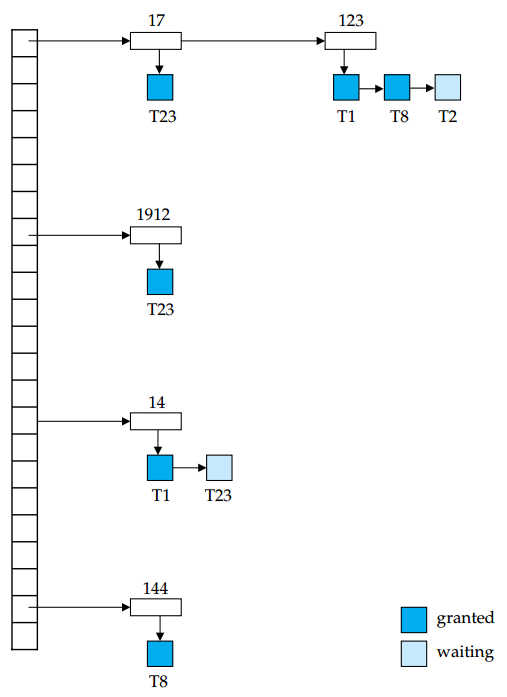
\includegraphics[width=0.8\linewidth]{locktable.png}
        \end{figure}
    
    \column{.5\textwidth} % Right column and width
    
        \textbf{Organização das requisições de cadeados}
        \begin{enumerate}
            \item Novas requisições entram no fim da fila de cada recurso e são concedidas quando forem compatíveis com as demais.
            \item Liberações (\emph{releases}) de cadeados removem a requisição da fila e as requisições pendentes são reavaliadas.
            \item Se um \emph{rollback} ou \emph{abort} é emitido, todo cadeado concedido e/ou pendente da transação é descartado.
        \end{enumerate}
    \end{columns}
\end{frame}

%------------------------------------------------

\begin{frame} % SLIDE 21
    \frametitle{2PL: Vantagens}

    \begin{columns}[c] % The "c" option specifies centered vertical alignment while the "t" option is used for top vertical alignment
    
        \column{.45\textwidth} % Left column and width
            \begin{figure}
                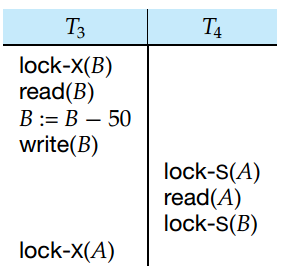
\includegraphics[width=0.8\linewidth]{example6.png}
            \end{figure}
        
        \column{.5\textwidth} % Right column and width
        
        A principal vantagem do 2PL (e a razão por ser a estratégia mais comum em sistemas distribuídos) é produzir um escalonamento que é garantido de ser serializável, isto é, reprodutível como se cada transação ocorresse uma após a outra.
    \end{columns}
    
\end{frame}


\begin{frame} % SLIDE 22
    \frametitle{2PL: Vantagens}

    \begin{figure}
        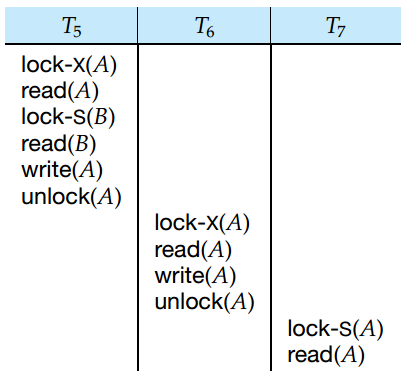
\includegraphics[width=0.6\linewidth]{example2.png}
    \end{figure}

\end{frame}

%------------------------------------------------

% \begin{frame} % SLIDE 23
% \frametitle{2PL: Desafios}
%     % TODO: acho que isso nao é verdade 2018-11-16 15:21:56
%     Nem todos os cenários de conflito podem ser serializados através do 2PL. 

%     \begin{example}{Exemplo 3}
%         % TODO: 2018-11-15 19:24:52
%     \end{example}

%     \medskip
%     \begin{example}{Exemplo 4}
%         % TODO: 2018-11-15 19:25:08
%         % TODO: opcional 2018-11-17 14:27:08
%     \end{example}

% \end{frame}

%------------------------------------------------

\begin{frame} % SLIDE 24
    \frametitle{2PL: Desafios}

    Ainda assim, 2PL oferece uma alternativa de serialização de conflitos mesmo na ausência de maiores informações. 

    \medskip
    \begin{theorem}[Serialização do 2PL]
        Caso haja uma transação \(T_{i}\) que não use \emph{2PL}, é possível coordenar as transações \(T_{j}\) de forma que, para cada par \( (Ti, \, Tj)\), não haja conflitos de serialização.
        % \item TODO: exemplo 5 2018-11-15 19:27:21
    \end{theorem}

    \medskip
    % TODO: inserir observação de que isso só ocorre quando o 2PL não é implementado por completo.
\end{frame}

%------------------------------------------------

\begin{frame} % SLIDE 25
    \frametitle{2PL: Desafios}

    \begin{columns}[c] % The "c" option specifies centered vertical alignment while the "t" option is used for top vertical alignment
    
        \column{.45\textwidth} % Left column and width
            \begin{figure}
                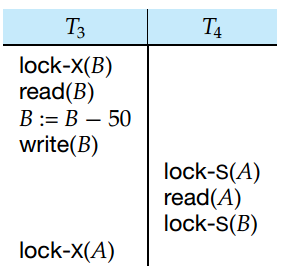
\includegraphics[width=0.8\linewidth]{example6.png}
            \end{figure}
        
        \column{.5\textwidth} % Right column and width
        
        2PL não necessariamente previne a existência de \emph{deadlocks}. Um exemplo clássico é o \emph{lock} cruzado, em que múltiplas transações necessitam do mesmo conjunto de recursos e cada uma segura o cadeado de um subconjunto dele, impedindo as demais de prosseguirem.
    \end{columns}
    
\end{frame}


\begin{frame} % SLIDE 26
    \frametitle{2PL: Desafios}

    \medskip
    2PL prevê apenas uma forma de resolução de tais conflitos: \emph{rollback} de ao menos uma das transações e descarte de suas permissões especiais.

    \medskip
    \medskip
    \begin{figure}
        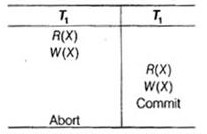
\includegraphics[width=0.4\linewidth]{example7.jpg}
    \end{figure}
\end{frame}


\begin{frame} % SLIDE 27
    \frametitle{2PL: Desafios}
    Por conta disto, há a possibilidade de "\emph{starvation}", cenário em que uma transação que necessita de acesso de escrita é repetidamente desfeita por conta da sequência de permissões de leitura concedidas sobre o mesmo recurso a outras transações.

    \medskip
    \begin{figure}
        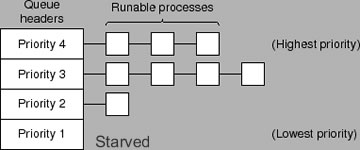
\includegraphics[width=0.8\linewidth]{starvation.jpg}
    \end{figure}
\end{frame}

%------------------------------------------------
\section{Q10: Variantes do 2PL}
% Discuta as variantes 2PL Normal, Conservativa, Estrita e Rigorosa.
%------------------------------------------------


\begin{frame} % SLIDE 28
    \frametitle{2PL: Estratégias}
    
    Caso ocorram \emph{deadlocks}, é papel do gerenciador de concorrência garantir a integridade, a consistência e a recuperação do sistema.
    
    \medskip
    Uma das consequências a serem evitadas é o \emph{rollback} em cascata, que é o cenário em que um \emph{deadlock} força várias transações interdependentes entre si a desfazerem suas operações. Existem algumas estratégias dentro do próprio 2PL para evitá-lo.
\end{frame}


\begin{frame} % SLIDE 29
    \frametitle{2PL: Estratégias}

    \begin{figure}
        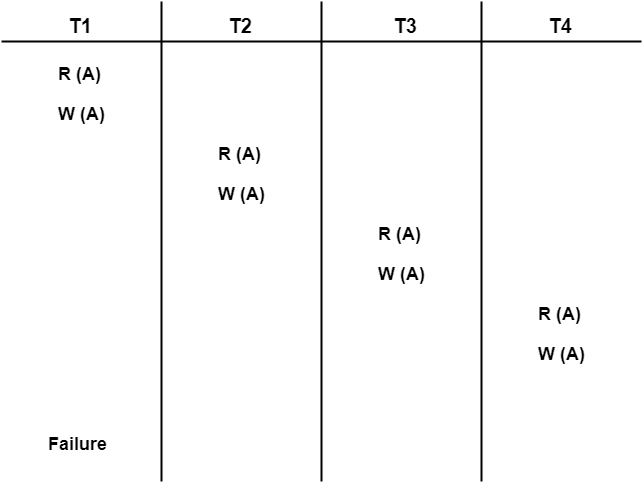
\includegraphics[width=0.8\linewidth]{example9.png}
    \end{figure}
\end{frame}
    

\begin{frame} % SLIDE 30
    \frametitle{2PL: Estratégias}
    \begin{block}{\textbf{Normal ou padrão}}
        Cada transação deve requerer seus cadeados quando necessitar dos recursos bloqueados e liberá-los logo em seguida. O mais simples de implementar, mas não garante um escalonamento livre de \emph{deadlocks}, ou um escalonamento estrito de recuperação.

        \begin{figure}
            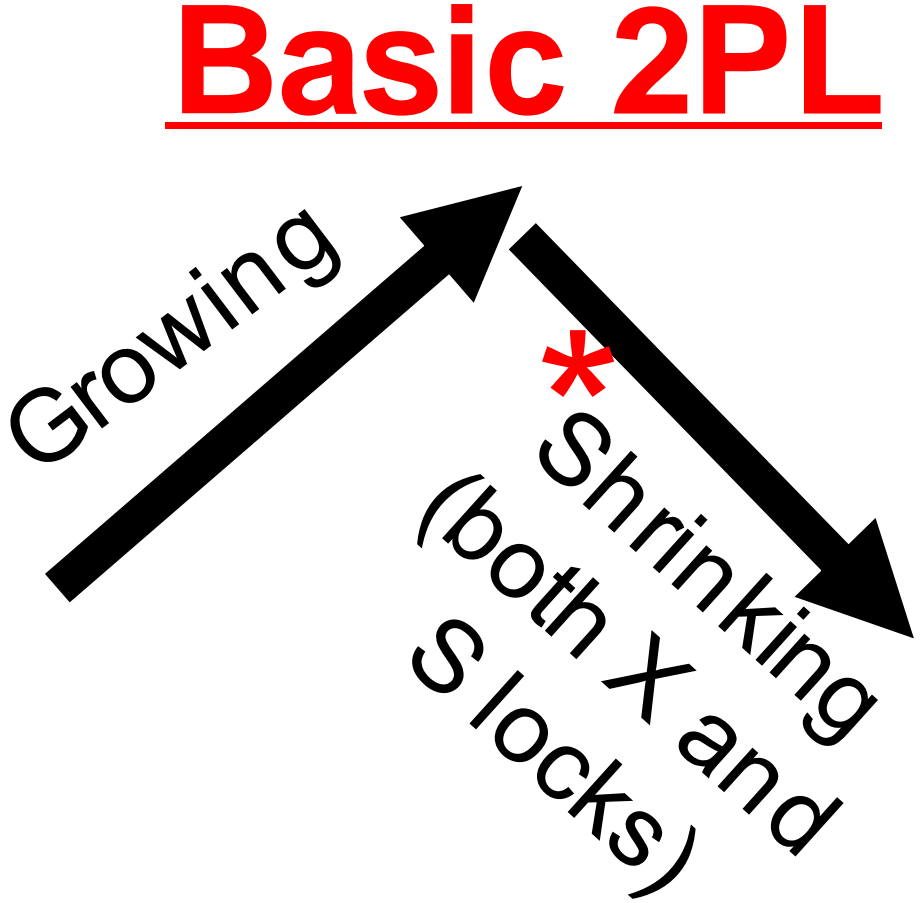
\includegraphics[width=0.4\linewidth]{basic2pl.png}
        \end{figure}
    \end{block}
\end{frame}

\begin{frame} % SLIDE 31
    \frametitle{2PL: Estratégias}
    
    \begin{block}{\textbf{Conservadora ou estática}}
        Cada transação deve requerer os cadeados antes de executar e liberá-los logo em seguida. A implementação exige conhecimento prévio do plano de execução, mas garante um escalonamento livre de \emph{deadlocks}. Ainda assim, não garante que ele seja estrito de recuperação, por permitir leituras sujas (\emph{dirty reads}).

        \medskip
        \begin{figure}
            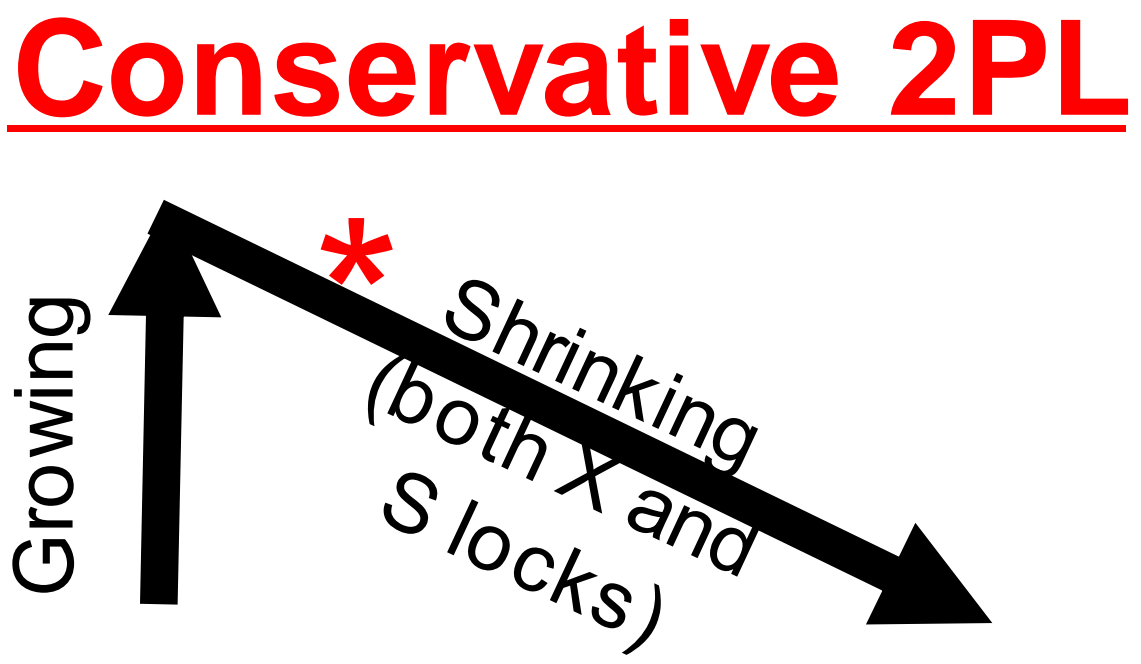
\includegraphics[width=0.55\linewidth]{conservative2pl.png}
        \end{figure}
    \end{block}
\end{frame}

%------------------------------------------------

\begin{frame} % SLIDE 32
    \frametitle{2PL: Estratégias}
    \begin{block}{\textbf{Estrita ou restrita}}
        Cada transação deve requerer seus cadeados exclusivos antes de iniciar a execução e segurá-los até que complete com sucesso ou aborte. A implementação exige conhecimento prévio do plano de execução, mas garante um escalonamento estrito de recuperação. \emph{Deadlocks} ainda podem ocorrer. Apesar disso, é uma das estratégias mais comuns (não só em SGBDs), graças aos algoritmos de detecção e tratamento de \emph{deadlocks}. Exemplos de SGBDs que o utilizam incluem o \emph{SQL Server} (Microsoft) e o \emph{DB2} (IBM).

        \medskip
        \begin{figure}
            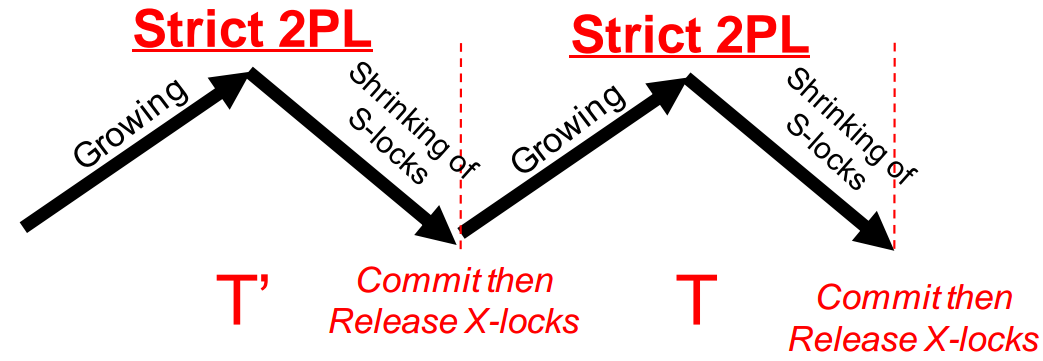
\includegraphics[width=0.6\linewidth]{strict2pl.png}
        \end{figure}
    \end{block}
\end{frame}


\begin{frame} % SLIDE 33
    \frametitle{2PL: Estratégias}
    \begin{block}{\textbf{Rigorosa}}
        Cada transação deve requerer todos os seus cadeados (exclusivos ou commpartilhados) antes de iniciar a execução e segurá-los até que complete ou aborte. As transações passam a ser serializadas pela ordem de \emph{commit}. A implementação exige conhecimento prévio do plano de execução, mas garante um escalonamento livre de \emph{deadlocks} e estrito de recuperação. Embora seja a implementação menos prática de todas, é uma estratégia bastante empregada por SGBDs.

        \medskip
        \begin{figure}
            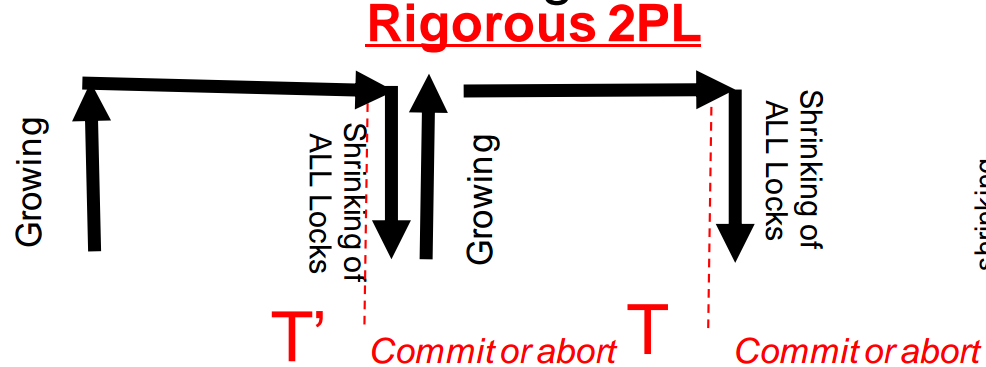
\includegraphics[width=0.65\linewidth]{rigorous2pl.png}
        \end{figure}
    \end{block}
\end{frame}

%------------------------------------------------
\section{Q11: Problemas e Prevenção}
% Explique e exemplifique os problemas de “\emph{deadlock}” e “\emph{starvation)“
% e os protocolos para as suas prevenções, mencionando detecção
% e recuperação de \emph{deadlocks} e esquema baseados em \emph{timestamps}
% ("\emph{wait-die)" e "\emph{wound-wait)").
%------------------------------------------------

%------------------------------------------------

\begin{frame} % SLIDE 34
    \frametitle{Demais estratégias de prevenção de \emph{deadlocks}}
    Outras estratégias de prevenção de \emph{deadlocks} incluem:

    \medskip
    \begin{block}{\textbf{Predeclaração}}
        Cada transação deve requerer todos os cadeados necessários antes mesmo de iniciar sua execução.
    \end{block}

    \medskip
    \begin{block}{\textbf{Ordenação parcial}}
        Cada transação só pode enviar requisições numa ordem parcial (menos estrita que a ordenação total para evitar \emph{overhead}).
    \end{block}
\end{frame}


\begin{frame} % SLIDE 35
    \frametitle{Demais estratégias de prevenção de \emph{deadlocks}}
    
    \begin{block}{\textbf{Timestamps não-preemptivos (\emph{wait-die})}}
        Transações antigas podem esperar recursos das posteriores, mas transações recentes são sempre desfeitas. O risco de \emph{starvation} é alto porque uma transação pode tomar \emph{rollback} repetidamente.
    \end{block}

    \medskip
    \begin{block}{\textbf{Timestamps preemptivos (\emph{wound-wait})}}
        Transações forçam \emph{rollback} das posteriores, mas as recentes podem esperar. O risco de \emph{starvation} é significativamente menor.
    \end{block}

\end{frame}

%------------------------------------------------

\begin{frame} % SLIDE 36
    \frametitle{Demais estratégias de prevenção de \emph{deadlocks}}

    \begin{itemize}
        \item Em ambos os casos de estratégias baseadas em \emph{timestamps}, a \emph{timestamp} original da transação é mantida caso ela seja executada novamente, de forma a prevenir \emph{starvation}.
    \end{itemize}

    \medskip
    \begin{block}{\textbf{\emph{Timeout}}}
        Se o cadeado não for concedido dentro de um certo intervalo de tempo, a transação é desfeita. Simples de implementar, porém a determinação do intervalo adequado é crucial para seu bom funcionamento.
    \end{block}
    
\end{frame}


%------------------------------------------------

\subsection{Detecção de \emph{deadlocks}}

\begin{frame} % SLIDE 37
    \frametitle{Detecção de \emph{deadlocks}}

    Os algoritmos mais eficazes de detecção de \emph{deadlocks} são os baseados no escalonamento de tarefas (\emph{jobshop scheduling problem} ou \emph{JSSP}).

    \medskip
    \begin{figure}
        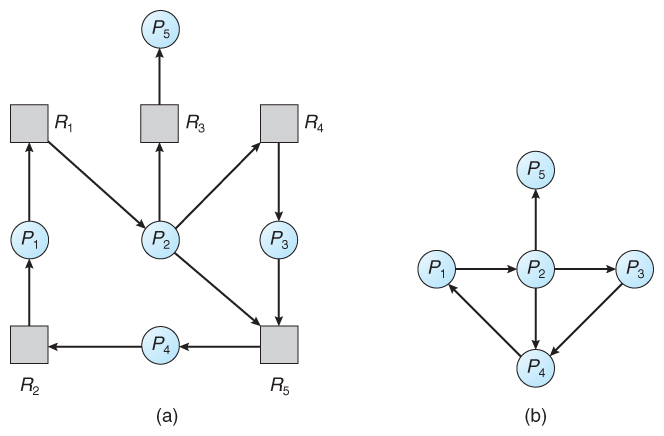
\includegraphics[width=0.75\linewidth]{deadlockdetection1.jpg}
    \end{figure}
\end{frame}


\begin{frame} % SLIDE 38
    \frametitle{Detecção de \emph{deadlocks}}
    % TODO: colocar em formato de demonstração matemática 2018-11-16 18:00:14

    \begin{theorem}
        O problema pode ser descrito por um conjunto de \(n\) transações \(\{\, J_{j} \, | \, 1 \, \leq \, j \, \leq \, n\, \}\) que requerem um conjunto de \(m\) recursos \(\{\, M_{r} \, | \, 1 \, \leq \, r \, \leq \, m\, \}\).

        \medskip
        Cada transação tem uma sequência própria de recursos a serem processados.

        \medskip
        O processamento da transação \(J_j\) na máquina \(M_r\) é chamada de operação \(O_{j_{r}}\).

        \medskip
        A operação \(O_{j_{r}}\) requer o uso exclusivo de Mr por uma duração ininterrupta \(p_{j_{r}}\), que é seu tempo de processamento.
        
    \end{theorem}

\end{frame}

%------------------------------------------------

\begin{frame} % SLIDE 39
    \frametitle{Detecção de \emph{deadlocks}}
    % TODO: colocar em formato de demonstração matemática 2018-11-16 18:00:14
    \begin{theorem}

        Um escalonamento eficaz é um conjunto de operações sequenciais \(\{\, c_{j_{r}} \, | \, 1 \, \leq \, j \, \leq \, n, \, 1 \, \leq \, r \, \leq \, m\, \}\) que satisfazem estes critérios.

        \medskip
        Caso haja um ciclo no escalonamento, então há um estado de \emph{deadlock} presente no escalonamento que precisa ser endereçado. O algoritmo deve buscar por ciclos frequentemente, para evitar \emph{rollbacks} em cascata.

    \end{theorem}

    \begin{figure}
        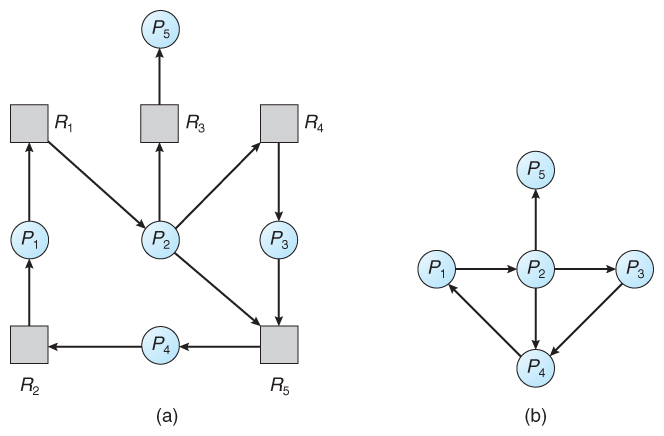
\includegraphics[width=0.5\linewidth]{deadlockdetection1.jpg}
    \end{figure}
\end{frame}


%------------------------------------------------

\begin{frame} % SLIDE 40
    \frametitle{Recuperação de \emph{deadlocks}}
    % TODO: dá para dividir este slide em 2 2018-11-17 14:40:46

    Quando um \emph{deadlock} é detectado, alguma transação deverá ser desfeita (\emph{rolled back}) para quebrá-lo. A seleção da vítima deve ser feita de forma a minimizar o prejuízo de tempo.

    \medskip
    A implementação mais simples é a do \emph{rollback} total, que aborta a transação e a desfaz completamente. Porém, esta operação pode ser muito custosa.

    \begin{figure}
        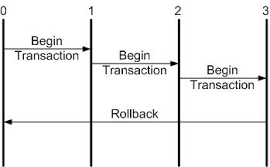
\includegraphics[width=0.5\linewidth]{completerollback.png}
    \end{figure}

\end{frame}


\begin{frame} % SLIDE 41
    \frametitle{Recuperação de \emph{deadlocks}}
    Uma implementação mais complicada, porém mais eficiente, é o \emph{rollback} parcial até que o \emph{deadlock} seja desfeito.

    \medskip
    Se a mesma transação é sempre escolhida como vítima, há o risco de \emph{starvation}.

    \medskip
    \begin{figure}
        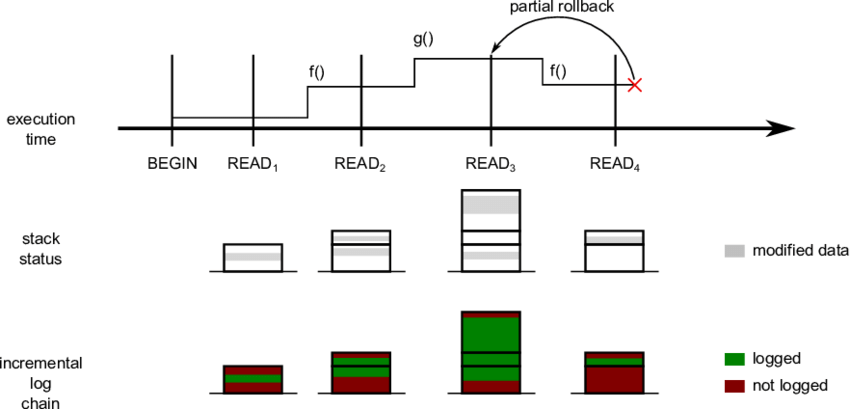
\includegraphics[width=0.8\linewidth]{partialrollback.png}
    \end{figure}

\end{frame}

%------------------------------------------------
\section{Q12: Métodos de Acesso Indexado}
% Discuta como os métodos de controle de concorrência baseado em locks
% consideram o uso de métodos de acesso indexados,
% comentando o nível de granularidade do lock através do índice;
%------------------------------------------------

%------------------------------------------------
\subsection{Granularidade múltipla}

\begin{frame} % SLIDE 42
    \frametitle{Granularidade múltipla}
    
    Idealmente, um SGBD deve oferecer às aplicações métodos de acesso indexado através de uma interface flexível de controle de acesso concorrente aos recursos.
    
    \medskip
    Uma das dimensões desta flexibilidade se dá através da granularidade dos cadeados, permitindo que pequenas porções de dados sejam aninhadas em porções maiores.
\end{frame}


\begin{frame} % SLIDE 43
    \frametitle{Acesso indexado}    
    A hierarquia de indexação do acesso a estas granularidades pode ser representada graficamente como uma árvore:
    
    \medskip
    \begin{figure}
        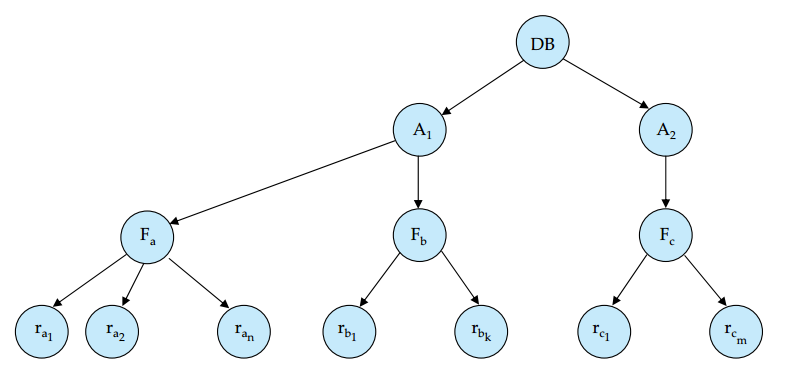
\includegraphics[width=0.8\linewidth]{granularitytree.png}
    \end{figure}
    
\end{frame}

%------------------------------------------------
    
\begin{frame} % SLIDE 44
    \frametitle{Acesso indexado}
    
    Quando uma transação requisita um cadeado explicitamente, o gerenciador de concorrência implicitamente aplica o cadeado a todos os recursos filhos daquele índice hierárquico.
    
    \medskip
    A granularidade do bloqueio, portanto, pode ocorrer em índices de:
    
    \medskip
    \begin{block}{Granularidade fina}
        Próxima às folhas da árvore, permitem maior grau de concorrência mas aumentam o custo computacional do gerenciamento (\emph{overhead}).
    \end{block}

    \medskip
    \begin{block}{Granularidade grossa}
        Próxima à raiz da árvore, simplificam o gerenciamento mas reduzem a capacidade de acessos concorrentes.
    \end{block}
\end{frame}


\begin{frame} % SLIDE 44
    \frametitle{Acesso indexado}

    Os índices da árvore de granularidade são:

    \medskip
    \begin{enumerate}
        \item base de dados \\~\\
        % TODO: adicionar detalhes 2018-11-17 14:46:09
        \item setor \\~\\
        % TODO: adicionar detalhes 2018-11-17 14:46:09
        \item arquivo \\~\\
        % TODO: adicionar detalhes 2018-11-17 14:46:09
        \item registro \\~\\
        % TODO: adicionar detalhes 2018-11-17 14:46:09
    \end{enumerate}
    
\end{frame}
    
%------------------------------------------------
    
\begin{frame} % SLIDE 45
    \frametitle{Tipos de intenção de cadeados}
    
    A partir do momento em que a granularidade múltipla passa a ser uma possibilidade oferecida pelo SGBD, os protocolos baseados em cadeados precisam passar a suportar três tipos adicionais de cadeados:

    \medskip
    \begin{block}{\textbf{\emph{lock IS} (intenção de compartilhamento)}}
        Requisita somente acessos concorrentes de leitura aos índices filhos do recurso.
    \end{block}

    \medskip
    \begin{block}{\textbf{\emph{lock IX} (intenção de exclusividade)}}
        Requisita acessos de escrita e leitura aos índices filhos do recurso. A distinção será feita numa granularidade mais fina.
    \end{block}

\end{frame}


\begin{frame} % SLIDE 46
    \frametitle{Tipos de intenção de cadeados}

    \begin{block}{\textbf{\emph{lock SIX} (compartilhado com intenção de exclusividade)}}
        Requer somente acesso de leitura aos índices filhos do recurso, mas acessos de escrita adicionais serão requeridos em granularidade mais fina. 
    \end{block}
    
    \medskip
    \medskip
    A vantagem de introduzir estes cadeados adicionais é a diminuição no tempo de resposta (\emph{overhead}) do gerenciamento de concorrência, já que eliminam a necessidade de checar todos os filhos do índice requisitado.
    
\end{frame}
    
%------------------------------------------------
    
\begin{frame} % SLIDE 47
    \frametitle{Matriz atualizada e compatibilidade de cadeados}

    \begin{table}
    \begin{tabular}{l l l l l l l l l l l l}
        \toprule

        \textbf{} && \textbf{IS} && \textbf{IX} && \textbf{S} && \textbf{SIX} && \textbf{X} \\

        \midrule

        \textbf{IS} && $\checkmark$ && $\checkmark$ && $\checkmark$ && $\checkmark$ && $\times$ \\
        \textbf{IX} && $\checkmark$ && $\checkmark$ && $\times$ && $\times$ && $\times$ \\
        \textbf{S} && $\checkmark$ && $\times$ && $\checkmark$ && $\times$ && $\times$ \\
        \textbf{SIX} && $\checkmark$ && $\times$ && $\times$ && $\times$ && $\times$ \\
        \textbf{X} && $\times$ && $\times$ && $\times$ && $\times$ && $\times$ \\

        \bottomrule
    \end{tabular}
    \caption{Cadeados adicionais oferecem opções intermediárias de controle de concorrência.}
    \end{table}
    
\end{frame}

%------------------------------------------------

\begin{frame} % SLIDE 48
    \frametitle{Esquematização dos cadeados sob granularidade múltipla}
    
    Uma transação pode obter cadeado de qualquer nó da árvore, desde que:

    \medskip
    \begin{enumerate}
        \item As regras da matriz atualizada de compatibilidade de cadeados sejam observadas.
        \item A raiz da árvore seja a primeira a ser reservada, e possa sê-la em qualquer modo.
        \item Um nó pode ser requisitado em nodo S ou IS somente se o nó pai dele estiver sob um cadeado IX ou IS pertencente à mesma transação.
    \end{enumerate}
\end{frame}


\begin{frame} % SLIDE 49
    \frametitle{Esquematização dos cadeados sob granularidade múltipla}

    \begin{enumerate}
        \setcounter{enumi}{3}
        \item Um nó pode ser requisitado em nodo X, SIX ou IX somente se o nó pai dele estiver sob um cadeado IX ou SIX pertencente à mesma transação.
        \item Um nó só pode ser requisitado se a transação não houver liberado nenhum nó anterior (ou seja, se está na fase de crescimento do 2PL).
        \item Um nó só pode ser liberado se nenhum de seus nós filhos estiver sob cadeado da mesma transação.
    \end{enumerate}
    
\end{frame}

%------------------------------------------------

\begin{frame} % SLIDE 50
    \frametitle{Esquematização dos cadeados sob granularidade múltipla}
    
    A fase de crescimento deve ocorrer sempre no sentido raiz $\Rightarrow$ folhas da árvore, enquanto a fase de retração deve ocorrer sempre no sentido oposto (folhas $\Rightarrow$ raiz).

    \medskip
    Se houver cadeados demais num mesmo nível da árvore, o gerenciador de concorrência poderá elevá-los a um nó de maior hierarquia. Este procedimento é chamado de escalação da granularidade do cadeado e deverá obedecer à matriz atualizada de compatibilidade.
\end{frame}


%------------------------------------------------

\section{Conclusão}

\begin{frame} % SLIDE 52
    \frametitle{Revisão}
    Em resumo, vimos nesta apresentação:
    
    \begin{enumerate}
        \item O que são cadeados e seus tipos
        \item Protocolos baseados em cadeados
        \item \emph{2PL} como ferramenta de serialização
        \begin{enumerate}
            \item Fase de crescimento e de retração
            \item Gerenciador de concorrência (\emph{lock manager})
            \item Tabela de cadeados (\emph{lock table})
        \end{enumerate}
        \item Variantes do \emph{2PL}
        \begin{enumerate}
            \item Normal (ou padrão)
            \item Conservadora (ou estática)
            \item Estrita (ou restrita)
            \item Rigorosa
        \end{enumerate}
        \item Prevenção de \emph{deadlocks}
        \item Detecção de \emph{deadlocks}
        \item Recuperação de \emph{deadlocks}
        \item Granularidade múltipla
        \item Métodos de acesso indexado
    \end{enumerate}

\end{frame}

\begin{frame} % SLIDE 52
    \frametitle{Conclusão}
    \begin{itemize}
        \item \emph{2PL} é um protocolo simples que promove serialização, mas é suscetível a \emph{deadlocks}.
        \item Variantes oferecem melhores escalonamentos a um custo maior de complexidade.
        \item Estratégias de prevenção, detecção e recuperação de \emph{deadlocks} ainda são necessárias.
        \item Uso da árvore de granularidade favorece o uso de métodos de acesso indexado com o \emph{2PL}.
    \end{itemize}

    % \medskip
    \begin{figure}
        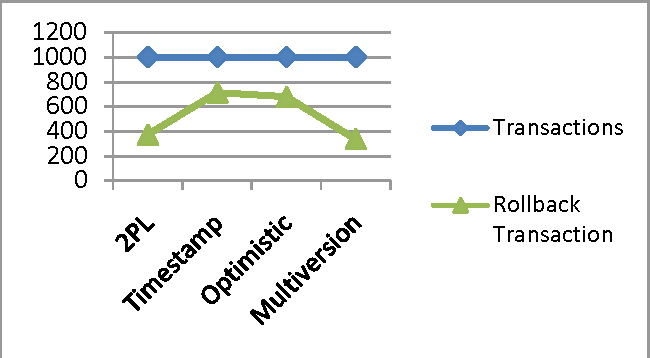
\includegraphics[width=0.53\linewidth]{conclusion.png}
    \end{figure}
\end{frame}

%------------------------------------------------

\section{Referências bibliográficas}

\begin{frame} % SLIDE 53
    \frametitle{Referências bibliográficas}
    \footnotesize{
    \begin{thebibliography}{99} % Beamer does not support BibTeX so references must be inserted manually as below
    % \bibitem[Smith, 2012]{p1} John Smith (2012)
        \bibitem[Silberschatz, 2010]{p1}
        Silberschatz, A., Korth, H. F., \& Sudarshan, S. (2010). Database system concepts (Vol. 4). New York: McGraw-Hill.

        \bibitem[Rawat, 2017]{p2}
        Rawat, U. (2017). Implementation of Locking in DBMS. Acessado a \date{25/11/2018} em https://www.geeksforgeeks.org/implementation-of-locking-in-dbms/.

        \bibitem[Porfirio, 2013]{p3}
        Porfirio, Alice \& Pellegrini, Alessandro \& Di Sanzo, Pierangelo \& Quaglia, Francesco. (2013). Transparent Support for Partial Rollback in Software Transactional Memories. 8097. 583-594. 10.1007/978-3-642-40047-6\_59. 

        \bibitem[Poddar, 2013]{p4}
        Poddar, Saumendra. (2003). SQL Server Transactions and Error Handling. Acessado a \date{25/11/2018} em https://www.codeproject.com/Articles/4451/SQL-Server-Transactions-and-Error-Handling.
    \end{thebibliography}
    }
\end{frame}


\begin{frame} % SLIDE 53
    \frametitle{Referências bibliográficas}
    \footnotesize{
    \begin{thebibliography}{99} % Beamer does not support BibTeX so references must be inserted manually as below

    \bibitem[Singhal, 2018]{p5}
        Singhal, Akshay. (2018). Cascading Schedule | Cascading Rollback | Cascadeless Schedule. Acessado a \date{25/11/2018} em https://www.gatevidyalay.com/cascading-schedule-cascading-rollback-cascadeless-schedule/.

        \bibitem[Pandey, 2018]{p6}
        Pandey, Anand. (2018). Transactions and Concurrency Control. Acessado a \date{25/11/2018} em https://gradeup.co/transactions-and-concurrency-control-i-4c5d9b27-c5a7-11e5-bcc4-bc86a005f7ba.

	    \bibitem[Difference between, 2018]{p7}
        Difference between. (2018). Difference between Deadlock and Starvation. Acessado a \date{25/11/2018} em http://www.differencebetween.info/difference-between-deadlock-and-starvation.

    \end{thebibliography}
    }
\end{frame}

%------------------------------------------------

\end{document} 
